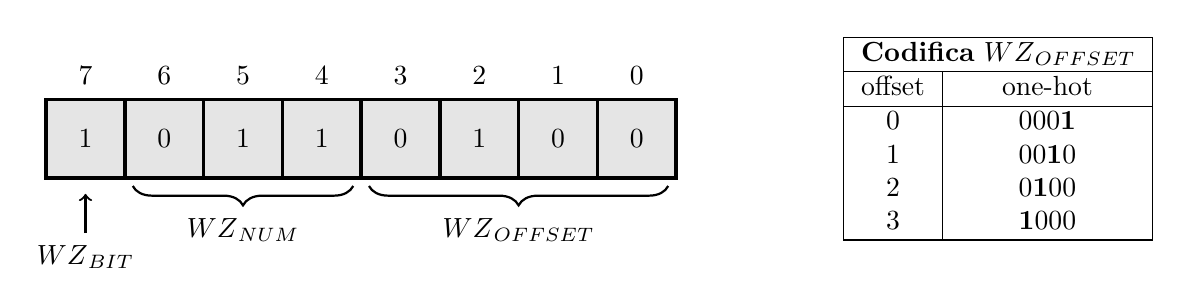
\begin{tikzpicture}[box/.style={fill=black!10, rectangle,draw=black, very thick, minimum size=1cm}]
	
	\foreach \i in {0,...,7} {
		\node at (8-\i-1,0.8){\i};
	}
	
	\foreach \y [count=\x] in {1,0,1,1,0,1,0,0} {
		\node[box] at (\x-1,0){\y};
	}

	\draw[decorate,decoration={brace, amplitude=7pt, raise=0pt, mirror}, thick] (0.6,-.6) -- node[below=8pt]{${WZ}_{NUM}$} (3.4,-.6);
	\draw[decorate,decoration={brace, amplitude=7pt, raise=0pt, mirror}, thick] (3.6,-.6) -- node[below=8pt]{${WZ}_{OFFSET}$} (7.4,-.6);
	\draw[->, thick] (0,-1.2) --  node[below=2pt,yshift=-2mm]{${WZ}_{BIT}$} (0,-.7);

	\node[text width=4cm, anchor=west, right] at (9.5,0) {	
		\begin{tabular}{ |c|c| }
		\hline
		\multicolumn{2}{|c|}{\textbf{Codifica ${WZ}_{OFFSET}$}} \\
		\hline
		offset & one-hot\\
		\hline
		0 & 000\textbf{1}\\
		1 & 00\textbf{1}0\\
		2 & 0\textbf{1}00\\
		3 & \textbf{1}000\\
		\hline
		\end{tabular}
	};
\end{tikzpicture}
